%!TEX program = xelatex
\documentclass[10pt]{beamer}

% Theme
\usetheme[progressbar=frametitle]{metropolis}
\usepackage{appendixnumberbeamer}

% Color palette (RA-inspired, finance-leaning)
\definecolor{StudyBlue}{HTML}{2E86C1}
\definecolor{StudyTeal}{HTML}{17A2B8}
\definecolor{StudyGrey}{HTML}{495057}
\definecolor{StudyLight}{HTML}{F8F9FA}
\definecolor{StudyGold}{HTML}{B8860B}

\setbeamercolor{primary}{bg=StudyBlue}
\setbeamercolor{secondary}{bg=StudyGrey}
\setbeamercolor{accent}{bg=StudyTeal}
\setbeamercolor{frametitle}{bg=StudyBlue, fg=white}
\setbeamercolor{progress bar}{fg=StudyTeal, bg=StudyGrey}

% Font sizing
\setbeamerfont{normal text}{size=\footnotesize}
\setbeamerfont{structure}{size=\footnotesize}
\setbeamerfont{frametitle}{size=\large}
\setbeamerfont{framesubtitle}{size=\scriptsize}

% Packages
\usepackage{amsmath}
\usepackage{amssymb}
\usepackage{amsthm}
\usepackage{mathtools}
\usepackage{graphicx}
\usepackage{tikz}
\usepackage{array}
\usepackage{booktabs}
\usepackage{tcolorbox}
\usepackage{bookmark}

% tcolorbox setup
\tcbuselibrary{theorems,skins}

% Spacing
\setlength{\parskip}{2pt}
\setlength{\itemsep}{1pt}

% Bullet styles
\setbeamercolor{item}{fg=StudyBlue}
\setbeamercolor{subitem}{fg=StudyBlue}
\setbeamercolor{subsubitem}{fg=StudyBlue}
\setbeamertemplate{itemize item}{\normalsize$\bullet$}
\setbeamertemplate{itemize subitem}{\large$\circ$}
\setbeamertemplate{itemize subsubitem}{\Large$\diamond$}

\setbeamercolor{enumerate item}{fg=StudyBlue}
\setbeamercolor{enumerate subitem}{fg=StudyBlue}
\setbeamercolor{enumerate subsubitem}{fg=StudyBlue}
\setbeamertemplate{enumerate item}{\textbf{\arabic{enumi}.}}
\setbeamertemplate{enumerate subitem}{\textbf{\alph{enumii})}}
\setbeamertemplate{enumerate subsubitem}{\textbf{\roman{enumiii}.}}

% Math shortcuts
\newcommand{\R}{\mathbb{R}}
\newcommand{\E}{\mathbb{E}}
\newcommand{\Var}{\mathrm{Var}}
\newcommand{\Cov}{\mathrm{Cov}}

% Box styles
\newtcolorbox{roundedbox}{
    colback=StudyBlue!5,
    colframe=StudyBlue!80,
    rounded corners,
    fonttitle=\bfseries
}

\newtcolorbox{definitionbox}[1][]{
    colback=StudyBlue!5,
    colframe=StudyBlue!80,
    fonttitle=\bfseries,
    title=Definition,
    before upper={
        \setbeamercolor{itemize item}{fg=StudyBlue}
        \setbeamercolor{itemize subitem}{fg=StudyBlue}
        \setbeamercolor{itemize subsubitem}{fg=StudyBlue}
    },
    #1
}

\newtcolorbox{theorembox}[1][]{
    colback=StudyTeal!5,
    colframe=StudyTeal!80,
    fonttitle=\bfseries,
    title=Theorem,
    before upper={
        \setbeamercolor{itemize item}{fg=StudyTeal}
        \setbeamercolor{itemize subitem}{fg=StudyTeal}
        \setbeamercolor{itemize subsubitem}{fg=StudyTeal}
    },
    #1
}

\newtcolorbox{examplebox}[1][]{
    colback=StudyGrey!5,
    colframe=StudyGrey!80,
    fonttitle=\bfseries,
    title=Example,
    before upper={
        \setbeamercolor{itemize item}{fg=StudyGrey}
        \setbeamercolor{itemize subitem}{fg=StudyGrey}
        \setbeamercolor{itemize subsubitem}{fg=StudyGrey}
    },
    #1
}

\newtcolorbox{notebox}[1][]{
    colback=black!5,
    colframe=black!90,
    fonttitle=\bfseries,
    fontupper=\footnotesize,
    title=Intuition,
    before upper={
        \setbeamercolor{itemize item}{fg=black}
        \setbeamercolor{itemize subitem}{fg=black}
        \setbeamercolor{itemize subsubitem}{fg=black}
    },
    #1
}

\newtcolorbox{proofbox}[1][]{
    colback=StudyLight,
    colframe=StudyGrey!50,
    fonttitle=\bfseries,
    title=Proof,
    before upper={
        \setbeamercolor{itemize item}{fg=StudyGrey}
        \setbeamercolor{itemize subitem}{fg=StudyGrey}
        \setbeamercolor{itemize subsubitem}{fg=StudyGrey}
    },
    #1
}

\newtcolorbox{keypoint}[1][]{
    colback=yellow!10,
    colframe=orange!80,
    fonttitle=\bfseries,
    title=Key Point,
    before upper={
        \setbeamercolor{itemize item}{fg=orange}
        \setbeamercolor{itemize subitem}{fg=orange}
        \setbeamercolor{itemize subsubitem}{fg=orange}
    },
    #1
}

\newtcolorbox{problembox}[1][]{
    colback=StudyGold!10,
    colframe=StudyGold!90,
    fonttitle=\bfseries,
    title=Problem,
    before upper={
        \setbeamercolor{itemize item}{fg=StudyGold}
        \setbeamercolor{itemize subitem}{fg=StudyGold}
        \setbeamercolor{itemize subsubitem}{fg=StudyGold}
    },
    #1
}

\title{Empirical Asset Pricing}
\subtitle{AP-01: CARA/Normal Equilibrium Pricing}
\author{Dr. Ian Helfrich}
\date{\today}

\begin{document}

\maketitle

\begin{frame}{From the Instructor}
\small
\begin{notebox}[title=A Quick Note]
\begin{itemize}
\item These are my own qualifier prep notes, written in full sentences on purpose.
\item I am an independent researcher (Georgia Tech PhD) and I have no current affiliation.
\item If a step feels fast, slow it down and work it line-by-line with me.
\end{itemize}
\end{notebox}
\end{frame}

\begin{frame}{Why This Problem Matters}
\small
\begin{roundedbox}
\textbf{Qualifier DNA}
\begin{itemize}
\item This is the canonical CARA/Normal equilibrium question.
\item It tests whether you can move from preferences to prices, fast and clean.
\item The same logic shows up in factor models, mean-variance, and SDF work.
\end{itemize}
\end{roundedbox}
\vspace{0.2cm}
\textbf{Goal for today:} you should be able to derive the price and the risk-free rate on a blank sheet, without looking anything up.
\end{frame}

\begin{frame}{What You Are Being Asked to Produce}
\small
\begin{problembox}[title=Deliverables]
\begin{itemize}
\item A demand function for each investor $h$.
\item A market-clearing price vector $p$.
\item A clear interpretation of the risk adjustment term.
\item A closed-form $R_f$ under common $\delta$, and the adjustment when $\delta_h$ differ.
\end{itemize}
\end{problembox}
\begin{notebox}[title=Exam Tip]
Write your final price as $p = \frac{1}{R_f}(\mu - \alpha\Sigma\theta)$ and then explain each term in one sentence. That earns partial credit even if algebra above is messy.
\end{notebox}
\end{frame}

\begin{frame}{Roadmap}
\small
\begin{enumerate}
\item \textbf{Problem and Setup}
\begin{itemize}
\item What is given, what is asked, and what we can safely ignore
\item Notation and market structure, kept consistent throughout
\end{itemize}
\item \textbf{Derivation}
\begin{itemize}
\item CARA/Normal certainty equivalent (the only real trick)
\item Individual demand, market clearing, and equilibrium price
\end{itemize}
\item \textbf{Risk-Free Rate and Interpretation}
\begin{itemize}
\item Common vs heterogeneous discounting
\item Economic meaning, plus the exact exam tips I use
\end{itemize}
\end{enumerate}
\end{frame}

\begin{frame}{How to Use These Notes}
\small
\begin{notebox}[title=Reading Advice]
\begin{itemize}
\item I go line-by-line. If a step feels quick, stop and check the algebra.
\item Every definition used later is stated here once. Use it as a reference.
\item The goal is not just the formula, but knowing why it must look that way.
\end{itemize}
\end{notebox}
\end{frame}

\begin{frame}{Qualifier Problem (BMGT840 Final 2024 Q1)}
\small
\begin{problembox}[title=Problem]
\begin{itemize}
\item Two dates, risky payoffs $X \sim N(\mu, \Sigma)$, supply $\theta$.
\item $H$ investors with CARA utilities
\vspace{4pt}
$u_0(c)=-e^{-\alpha_h c}, \quad u_1(c)=-\delta_h e^{-\alpha_h c}.$
\item Show: $p = \frac{1}{R_f}(\mu - \alpha\,\Sigma\theta)$.
\item Interpret the risk adjustment term.
\item Derive $R_f$ when $\delta_h$ are common; then when they differ.
\end{itemize}
\end{problembox}
\end{frame}

\begin{frame}{Setup and Notation}
\small
\begin{roundedbox}
\textbf{Given}
\begin{itemize}
\item Risky payoffs $X \in \R^n$, $X \sim N(\mu, \Sigma)$.
\item Price vector $p$ at $t=0$, risk-free return $R_f$.
\item Supply vector $\theta$.
\item Aggregate $t=0$ endowment $c_0$.
\end{itemize}
\end{roundedbox}
\vspace{0.3cm}
\textbf{Investor $h$ chooses:}
\begin{itemize}
\item $c_{0h}$, risky holdings $\theta_h$, risk-free holdings $B_h$.
\item Date-0 budget: $c_{0h}+p'\theta_h+(1/R_f)B_h=w_{0h}$.
\item Date-1 consumption: $c_{1h}=\theta_h'X+B_h$.
\end{itemize}
\vspace{0.2cm}
\textbf{Note:} I will keep all vectors as column vectors, and I will write every transpose.
\end{frame}

\begin{frame}{Equilibrium Conditions (Keep These Visible)}
\small
\begin{roundedbox}
\textbf{Market Clearing}
\begin{itemize}
\item Risky assets: $\sum_{h=1}^H \theta_h = \theta$.
\item Risk-free asset: $\sum_{h=1}^H B_h = 0$.
\item Date-0 goods: $\sum_{h=1}^H c_{0h} = c_0$.
\end{itemize}
\end{roundedbox}
\vspace{0.2cm}
\begin{notebox}[title=Why this matters]
Every equilibrium price comes from these three conditions plus the FOCs.
\end{notebox}
\end{frame}

\begin{frame}{Timeline (Two-Date Economy)}
\small
\begin{center}
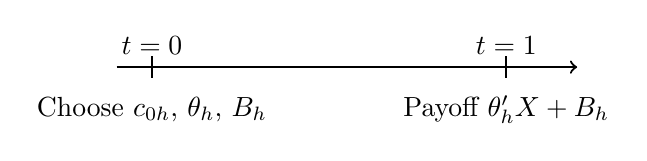
\begin{tikzpicture}[scale=0.9]
\draw[->, thick] (-0.5,0) -- (6,0);
\node at (0,0.3) {$t=0$};
\node at (5,0.3) {$t=1$};
\draw[thick] (0,0.15) -- (0,-0.15);
\draw[thick] (5,0.15) -- (5,-0.15);

\node[align=center] at (0,-0.6) {Choose $c_{0h}$, $\theta_h$, $B_h$};
\node[align=center] at (5,-0.6) {Payoff $\theta_h'X+B_h$};
\end{tikzpicture}
\end{center}
\end{frame}

\begin{frame}{Key Lemma: CARA/Normal Certainty Equivalent}
\small
\begin{theorembox}[title=Certainty Equivalent]
If $Y \sim N(m,v)$ and utility is $-\exp(-\alpha Y)$, then maximizing
$\E[-e^{-\alpha Y}]$ is equivalent to maximizing
\[\text{CE} = m - \frac{\alpha}{2}v.\]
\end{theorembox}
\vspace{0.2cm}
\begin{proofbox}[title=Proof Sketch]
\small
\begin{itemize}
\item $\E[e^{-\alpha Y}] = \exp(-\alpha m + \tfrac{\alpha^2}{2}v)$.
\item Exponential is monotone, so maximize $-\alpha m + \tfrac{\alpha^2}{2}v$.
\item Equivalent to maximize $m - \tfrac{\alpha}{2}v$.
\item This lemma is the workhorse for the rest of the course.
\end{itemize}
\end{proofbox}
\end{frame}

\begin{frame}{Lemma in Full (Line-by-Line)}
\small
\begin{proofbox}[title=Full Derivation]
\begin{align*}
\E[-e^{-\alpha Y}] &= -\E\left[\exp(-\alpha Y)\right] \\
&= -\exp\left(-\alpha m + \frac{\alpha^2}{2}v\right) \\
&\text{(normal MGF)}.
\end{align*}
Maximizing this is equivalent to maximizing
\[-\alpha m + \tfrac{\alpha^2}{2}v\]
which is equivalent to maximizing
\[m - \tfrac{\alpha}{2}v.\]
\end{proofbox}
\begin{notebox}[title=Practical Note]
If you memorize one formula from this course, make it this one.
\end{notebox}
\end{frame}

\begin{frame}{Step 1: Express $c_{1h}$ in Terms of $\theta_h$}
\small
\textbf{Date-0 budget:}
\[c_{0h}+p'\theta_h+(1/R_f)B_h=w_{0h} \Rightarrow B_h=R_f(w_{0h}-c_{0h}-p'\theta_h).\]
\vspace{0.2cm}
\textbf{Date-1 consumption:}
\begin{align*}
 c_{1h} &= \theta_h'X + B_h \\
 &= \theta_h'X + R_f(w_{0h}-c_{0h}-p'\theta_h) \\
 &= R_f(w_{0h}-c_{0h}) + \theta_h'(X - R_f p).
\end{align*}
\end{frame}

\begin{frame}{Step 2: Mean and Variance of $c_{1h}$}
\small
\textbf{Mean}
\[\E[c_{1h}] = R_f(w_{0h}-c_{0h}) + \theta_h'(\mu - R_f p).\]
\textbf{Variance}
\begin{align*}
\Var(c_{1h}) &= \Var(\theta_h'X) \\
&= \theta_h'\Sigma\,\theta_h.
\end{align*}
\begin{notebox}[title=Note]
Risk-free terms are constants, so they drop out of variance.
\end{notebox}
\end{frame}

\begin{frame}{Step 3: Certainty Equivalent Objective}
\small
Using the lemma:
\begin{align*}
\text{CE}_h &= \E[c_{1h}] - \frac{\alpha_h}{2}\Var(c_{1h}) \\
&= R_f(w_{0h}-c_{0h}) + \theta_h'(\mu - R_f p)
 - \frac{\alpha_h}{2}\theta_h'\Sigma\theta_h.
\end{align*}
\textbf{Choice variable:} $\theta_h$ (holding $c_{0h}$ fixed).
\end{frame}

\begin{frame}{Step 4: First-Order Condition}
\small
\textbf{Differentiate with respect to $\theta_h$:}
\begin{align*}
\frac{\partial}{\partial \theta_h} \theta_h'(\mu - R_f p) &= \mu - R_f p, \\
\frac{\partial}{\partial \theta_h} \Big(\tfrac{\alpha_h}{2}\theta_h'\Sigma\theta_h\Big)
&= \alpha_h \Sigma \theta_h.
\end{align*}
\textbf{Pause:} we use the symmetry of $\Sigma$ here.
\textbf{FOC:}
\[\mu - R_f p - \alpha_h \Sigma \theta_h = 0.\]
\end{frame}

\begin{frame}{Step 5: Individual Demand}
\small
Solve the FOC:
\begin{align*}
\alpha_h \Sigma\theta_h &= \mu - R_f p \\
\theta_h &= \frac{1}{\alpha_h} \Sigma^{-1}(\mu - R_f p).
\end{align*}
\begin{keypoint}[title=Key Insight]
Demand is linear in expected excess payoff and inversely proportional to risk aversion.
\end{keypoint}
\end{frame}

\begin{frame}{Sanity Check: Shapes and Units}
\small
\begin{roundedbox}
\textbf{Dimensions}
\begin{itemize}
\item $\mu$ and $p$ are $n \times 1$ vectors.
\item $\Sigma$ is $n \times n$.
\item $\theta_h$ is $n \times 1$.
\item Therefore $\Sigma\theta_h$ is $n \times 1$, matching $\mu - R_f p$.
\end{itemize}
\end{roundedbox}
\vspace{0.2cm}
\begin{notebox}[title=Why I check this]
On quals, a quick dimension check catches half of algebra mistakes.
\end{notebox}
\end{frame}

\begin{frame}{Step 6: Market Clearing}
\small
\textbf{Aggregate supply:}
\[\sum_{h=1}^H \theta_h = \theta.\]
Substitute individual demands:
\begin{align*}
\theta &= \sum_{h=1}^H \frac{1}{\alpha_h} \Sigma^{-1}(\mu - R_f p) \\
&= T\,\Sigma^{-1}(\mu - R_f p),
\end{align*}
where $T = \sum_{h=1}^H 1/\alpha_h$ is aggregate risk tolerance.
\end{frame}

\begin{frame}{Step 7: Equilibrium Price}
\small
Multiply by $\Sigma$:
\[\Sigma\theta = T(\mu - R_f p).\]
Solve for $p$:
\begin{align*}
\mu - R_f p &= \frac{1}{T}\Sigma\theta, \\
R_f p &= \mu - \alpha\,\Sigma\theta,
\end{align*}
where $\alpha = 1/T$ is aggregate risk aversion.
\vspace{0.2cm}
\begin{keypoint}
\[p = \frac{1}{R_f}(\mu - \alpha\,\Sigma\theta).\]
\end{keypoint}
\end{frame}

\begin{frame}{Notation Pitfall: Aggregate Risk Aversion}
\small
\begin{notebox}[title=Be Precise]
Some notes define
\[T = \sum_h \frac{1}{\alpha_h} \quad \text{and} \quad \alpha = \frac{1}{T}.\]
Other notes (and some exams) write $\alpha = \sum_h \alpha_h$.\\
\textbf{Always check the definition in the problem statement.}
Your algebra is right either way, but the symbol may differ.
\end{notebox}
\end{frame}

\begin{frame}{One-Asset Sanity Check}
\small
Assume $n=1$, so $\Sigma=\sigma^2$ and supply is $\theta$.
\begin{align*}
p &= \frac{1}{R_f}(\mu - \alpha\sigma^2\theta).
\end{align*}
\textbf{Interpretation:}
\begin{itemize}
\item Higher $\mu$ raises price.
\item Higher risk ($\sigma^2$) lowers price.
\item More supply $\theta$ lowers price (risk must be absorbed).
\end{itemize}
\begin{notebox}[title=Exam Tip]
If your formula fails this one-asset check, something went wrong upstream.
\end{notebox}
\end{frame}

\begin{frame}{Interpretation: The Risk Adjustment Term}
\small
\textbf{Price decomposition:}
\[p = \frac{1}{R_f}\mu - \frac{\alpha}{R_f}\Sigma\theta.\]
\begin{notebox}[title=Economic Meaning]
\begin{itemize}
\item $\mu$ is the expected payoff.
\item $(\Sigma\theta)_i = \Cov(X_i,\theta'X)$ is each asset's covariance with aggregate risk.
\item Larger covariance $\Rightarrow$ larger discount $\Rightarrow$ lower price.
\end{itemize}
\end{notebox}
\end{frame}

\begin{frame}{Risk-Free Rate: Common Discount Factor}
\small
Assume $\delta_h=\delta$ for all $h$.
\vspace{0.2cm}
\textbf{Aggregate consumption at $t=1$:}
\[c_1=\theta'X.\]
\textbf{SDF:}
\[m=\delta\exp\{-\alpha(c_1-c_0)\}.\]
\textbf{Risk-free pricing:}
\[\frac{1}{R_f}=\E[m].\]
\end{frame}

\begin{frame}{Risk-Free Rate: Identify Mean and Variance}
\small
Let $c_1 = \theta'X$.
Since $X \sim N(\mu,\Sigma)$, we have
\begin{align*}
\E[c_1] &= \theta'\mu, \\\\
\Var(c_1) &= \theta'\Sigma\theta.
\end{align*}
Therefore $c_1 \sim N(\theta'\mu,\theta'\Sigma\theta)$.
\begin{notebox}[title=Why this matters]
We need the mean and variance to apply the normal MGF.
\end{notebox}
\end{frame}

\begin{frame}{Risk-Free Rate: Step-by-Step Evaluation}
\small
Since $c_1=\theta'X$ and $X \sim N(\mu,\Sigma)$:
\begin{align*}
\E[m] &= \delta\,e^{\alpha c_0}\E\left[\exp\{-\alpha\theta'X\}\right] \\
&= \delta\,e^{\alpha c_0}\exp\left(-\alpha\theta'\mu
+\tfrac{\alpha^2}{2}\theta'\Sigma\theta\right).
\end{align*}
Therefore:
\[R_f=\frac{1}{\delta}\exp\left(\alpha\theta'\mu-\alpha c_0-\tfrac{\alpha^2}{2}\theta'\Sigma\theta\right).\]
\end{frame}

\begin{frame}{Risk-Free Rate: Two Quick Checks}
\small
\begin{examplebox}[title=Check 1: No Aggregate Risk]
If $\theta=0$, then $c_1$ is non-random and
\[R_f = \frac{1}{\delta} e^{-\alpha c_0}.\]
This is exactly the CARA discounting of certain consumption.
\end{examplebox}
\vspace{0.2cm}
\begin{examplebox}[title=Check 2: More Aggregate Risk]
If $\theta'\Sigma\theta$ rises, $R_f$ falls. Safe claims become more valuable.
\end{examplebox}
\end{frame}

\begin{frame}{Comparative Statics for $R_f$}
\small
From
\[R_f=\frac{1}{\delta}\exp\left(\alpha\theta'\mu-\alpha c_0-\tfrac{\alpha^2}{2}\theta'\Sigma\theta\right):\]
\begin{itemize}
\item Higher $\theta'\mu$ \textbf{increases} $R_f$.
\item Higher $\delta$ \textbf{reduces} $R_f$ (more patient investors).
\item Higher $c_0$ \textbf{reduces} $R_f$ (more current endowment).
\item Higher risk term $\alpha^2\theta'\Sigma\theta$ \textbf{reduces} $R_f$.
\end{itemize}
\end{frame}

\begin{frame}{Heterogeneous Discount Factors: Key Idea}
\small
When $\delta_h$ differ, a representative discount factor is a
\textbf{risk-tolerance-weighted geometric mean}.
\begin{notebox}[title=Plan]
\begin{itemize}
\item Solve planner problems at $t=0$ and $t=1$.
\item Derive $m(\omega)=\Lambda_1(\omega)/\Lambda_0$.
\item Identify an effective $\bar{\delta}$.
\end{itemize}
\end{notebox}
\end{frame}

\begin{frame}{Heterogeneous $\delta_h$: Planner FOCs}
\small
\textbf{At $t=0$:}
\[\lambda_h \alpha_h e^{-\alpha_h c_{0h}}=\Lambda_0.\]
\textbf{At $t=1$ in state $\omega$:}
\[\lambda_h \delta_h \alpha_h e^{-\alpha_h c_{1h}(\omega)}=\Lambda_1(\omega).\]
\textbf{Solve:}
\begin{align*}
 c_{0h} &= -\frac{1}{\alpha_h}\ln\left(\frac{\Lambda_0}{\lambda_h\alpha_h}\right), \\
c_{1h}(\omega) &= -\frac{1}{\alpha_h}\ln\left(\frac{\Lambda_1(\omega)}{\lambda_h\delta_h\alpha_h}\right).
\end{align*}
\end{frame}

\begin{frame}{Solve for Multipliers (Step-by-Step)}
\small
Let $T = \sum_h 1/\alpha_h$ and define
\[K_0 = \sum_h \frac{1}{\alpha_h} \ln(\lambda_h\alpha_h).\]
Summing $c_{0h}$ over $h$ gives
\begin{align*}
c_0 &= -T\ln\Lambda_0 + K_0, \\\\
\ln\Lambda_0 &= \frac{K_0 - c_0}{T}.
\end{align*}
Define
\[K_1 = \sum_h \frac{1}{\alpha_h} \ln(\lambda_h\delta_h\alpha_h).\]
Then
\begin{align*}
c_1(\omega) &= -T\ln\Lambda_1(\omega) + K_1, \\\\
\ln\Lambda_1(\omega) &= \frac{K_1 - c_1(\omega)}{T}.
\end{align*}
\end{frame}

\begin{frame}{Heterogeneous $\delta_h$: Effective Discounting}
\small
Let $T=\sum_h 1/\alpha_h$ and define
\[\bar{\delta}=\exp\left(\frac{\sum_h (1/\alpha_h)\ln\delta_h}{\sum_h (1/\alpha_h)}\right).\]
Then the SDF is
\[m(\omega)=\bar{\delta}\exp\{-\alpha(c_1(\omega)-c_0)\}.\]
\textbf{Risk-free rate:}
\[R_f=\frac{1}{\bar{\delta}}\exp\left(\alpha\theta'\mu-\alpha c_0-\tfrac{\alpha^2}{2}\theta'\Sigma\theta\right).\]
\end{frame}

\begin{frame}{Interpretation of $\bar{\delta}$}
\small
\begin{notebox}[title=Economic Meaning]
\begin{itemize}
\item Investors with lower risk aversion receive more weight.
\item $\bar{\delta}$ is a geometric mean, not an arithmetic mean.
\item If all $\delta_h$ are equal, $\bar{\delta} = \delta$.
\end{itemize}
\end{notebox}
\end{frame}

\begin{frame}{Key Takeaways}
\small
\begin{keypoint}
\begin{itemize}
\item CARA/Normal reduces equilibrium pricing to mean-variance logic.
\item Price = expected payoff minus a covariance-based risk adjustment.
\item $R_f$ depends on expected aggregate payoff, patience, and aggregate risk.
\item Heterogeneous $\delta_h$ aggregate via a risk-tolerance-weighted geometric mean.
\end{itemize}
\end{keypoint}
\end{frame}

\begin{frame}{Practice Variant}
\small
\begin{examplebox}[title=Practice]
Assume one risky asset and add a second risk-free asset with payoff 2 and price $2/R_f$.
\begin{itemize}
\item Show the risky-asset price formula is unchanged.
\item Explain why the second risk-free asset is redundant.
\end{itemize}
\end{examplebox}
\end{frame}

\begin{frame}{Common Pitfalls}
\small
\begin{notebox}[title=Common Pitfalls]
\begin{itemize}
\item Forgetting the price term $R_f p$ in the FOC.
\item Mixing up aggregate risk tolerance $T$ and risk aversion $\alpha$.
\item Dropping transposes in quadratic forms (use $\theta'\Sigma\theta$).
\item Ignoring the role of $c_0$ in $R_f$.
\end{itemize}
\end{notebox}
\end{frame}

\end{document}
